\section{Example Objects}

To evaluate our tool's capabilities and to explore new points in the design space, we fabricated a set of five prototype objects designed using the tool.

\subsection{Touch-sensitive Toys}

\begin{figure}[h]
\centering
    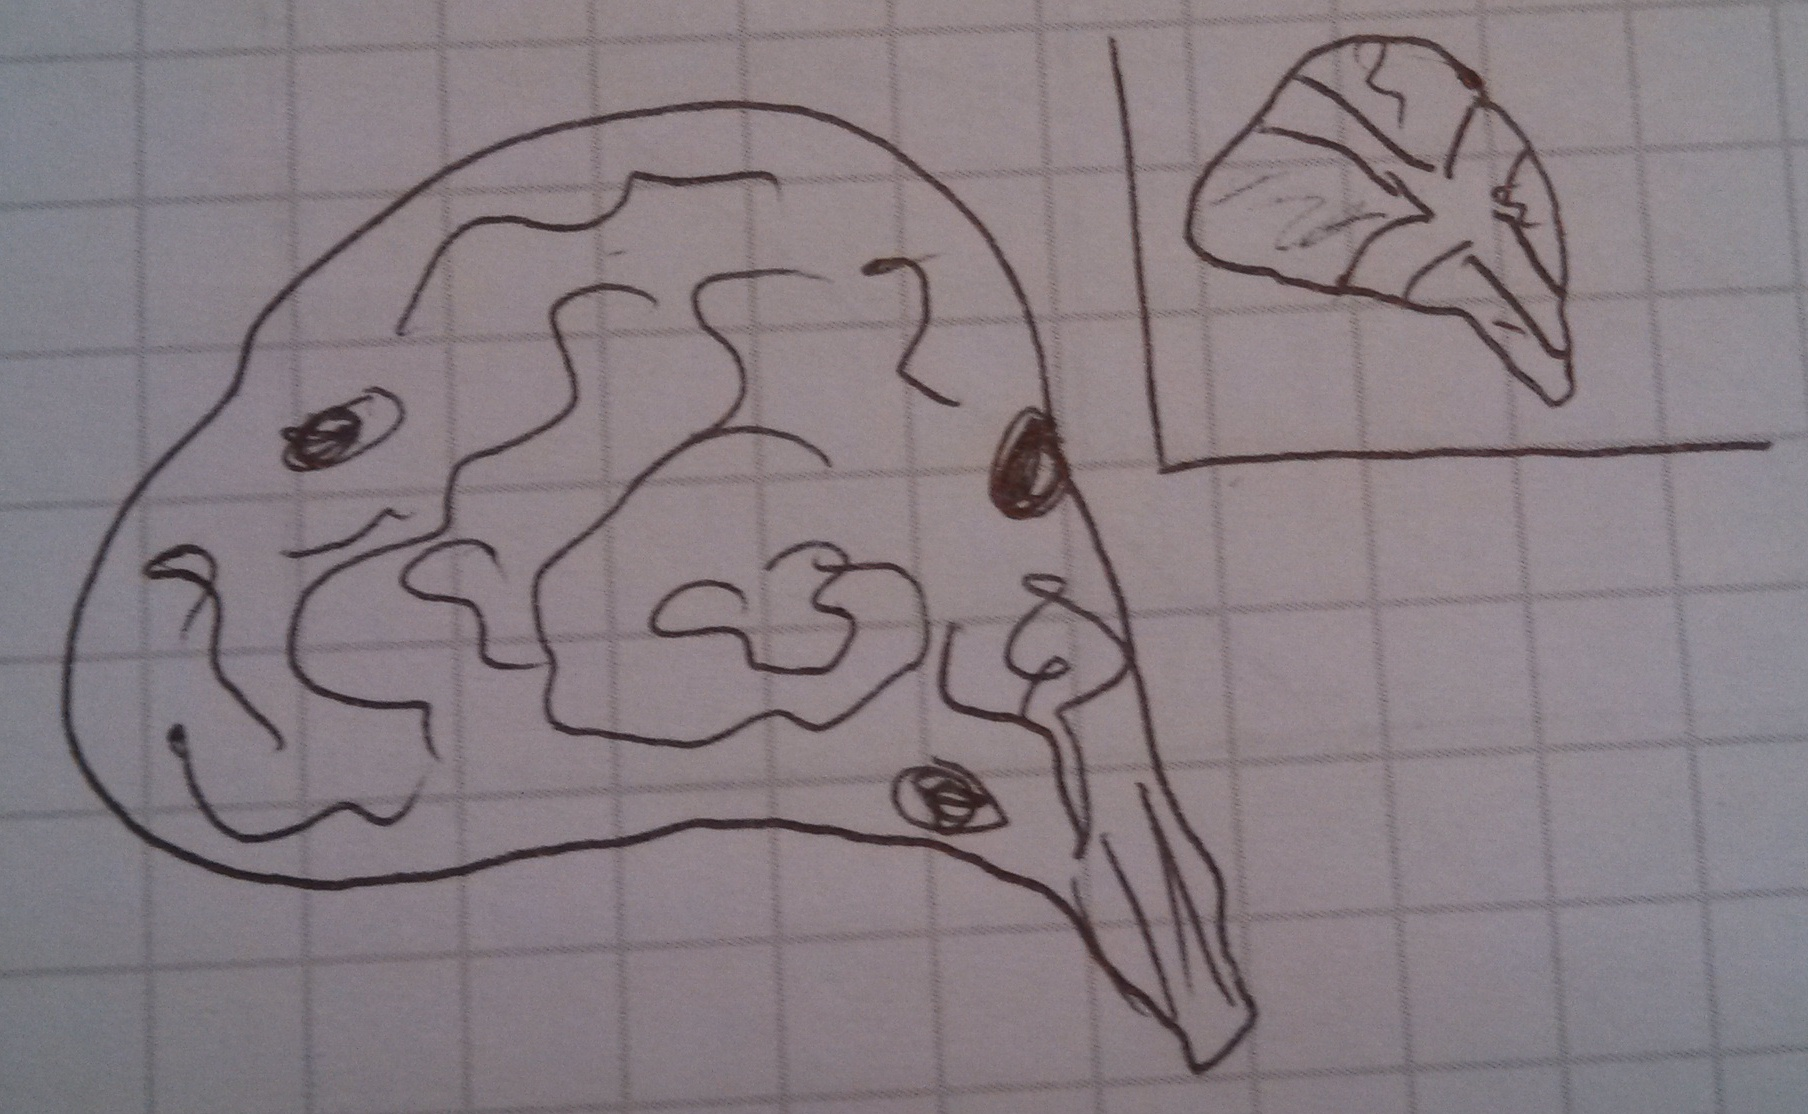
\includegraphics[width=3.4in]{figures/placeholder/brain.jpg}
\caption{A touch-sensitive brain whose tubes are filled with conductive paint.  Sensing is done on a single wire via SFCS.  Inset shows the internal structure of the tubes generated by our design tool.}
\label{fig:toys}
\end{figure}

We created a set of touch-sensitive toys and a companion app, reminiscent of the boat application in \cite{Harrison-acoustic}.  The brain, rabbit, and boat each have several distinct touch points on their surfaces.  These touch points are connected by an interior star topology of tubes filled with conductive copper paint, and touch sensing is performed via a single wire and SFCS (see Figure \ref{fig:toys}).  We built a smart base which can distinguish between the toys and also determine which toy is mounted: since each toy and each gesture has a distinct capacitive signature, we use a simple classifier trained to detect both toy and gesture based on profile.  All components were fabricated on a Makerbot Replicator 2.

\subsection{Breathing Bunny}

\begin{figure}[h]
\centering
    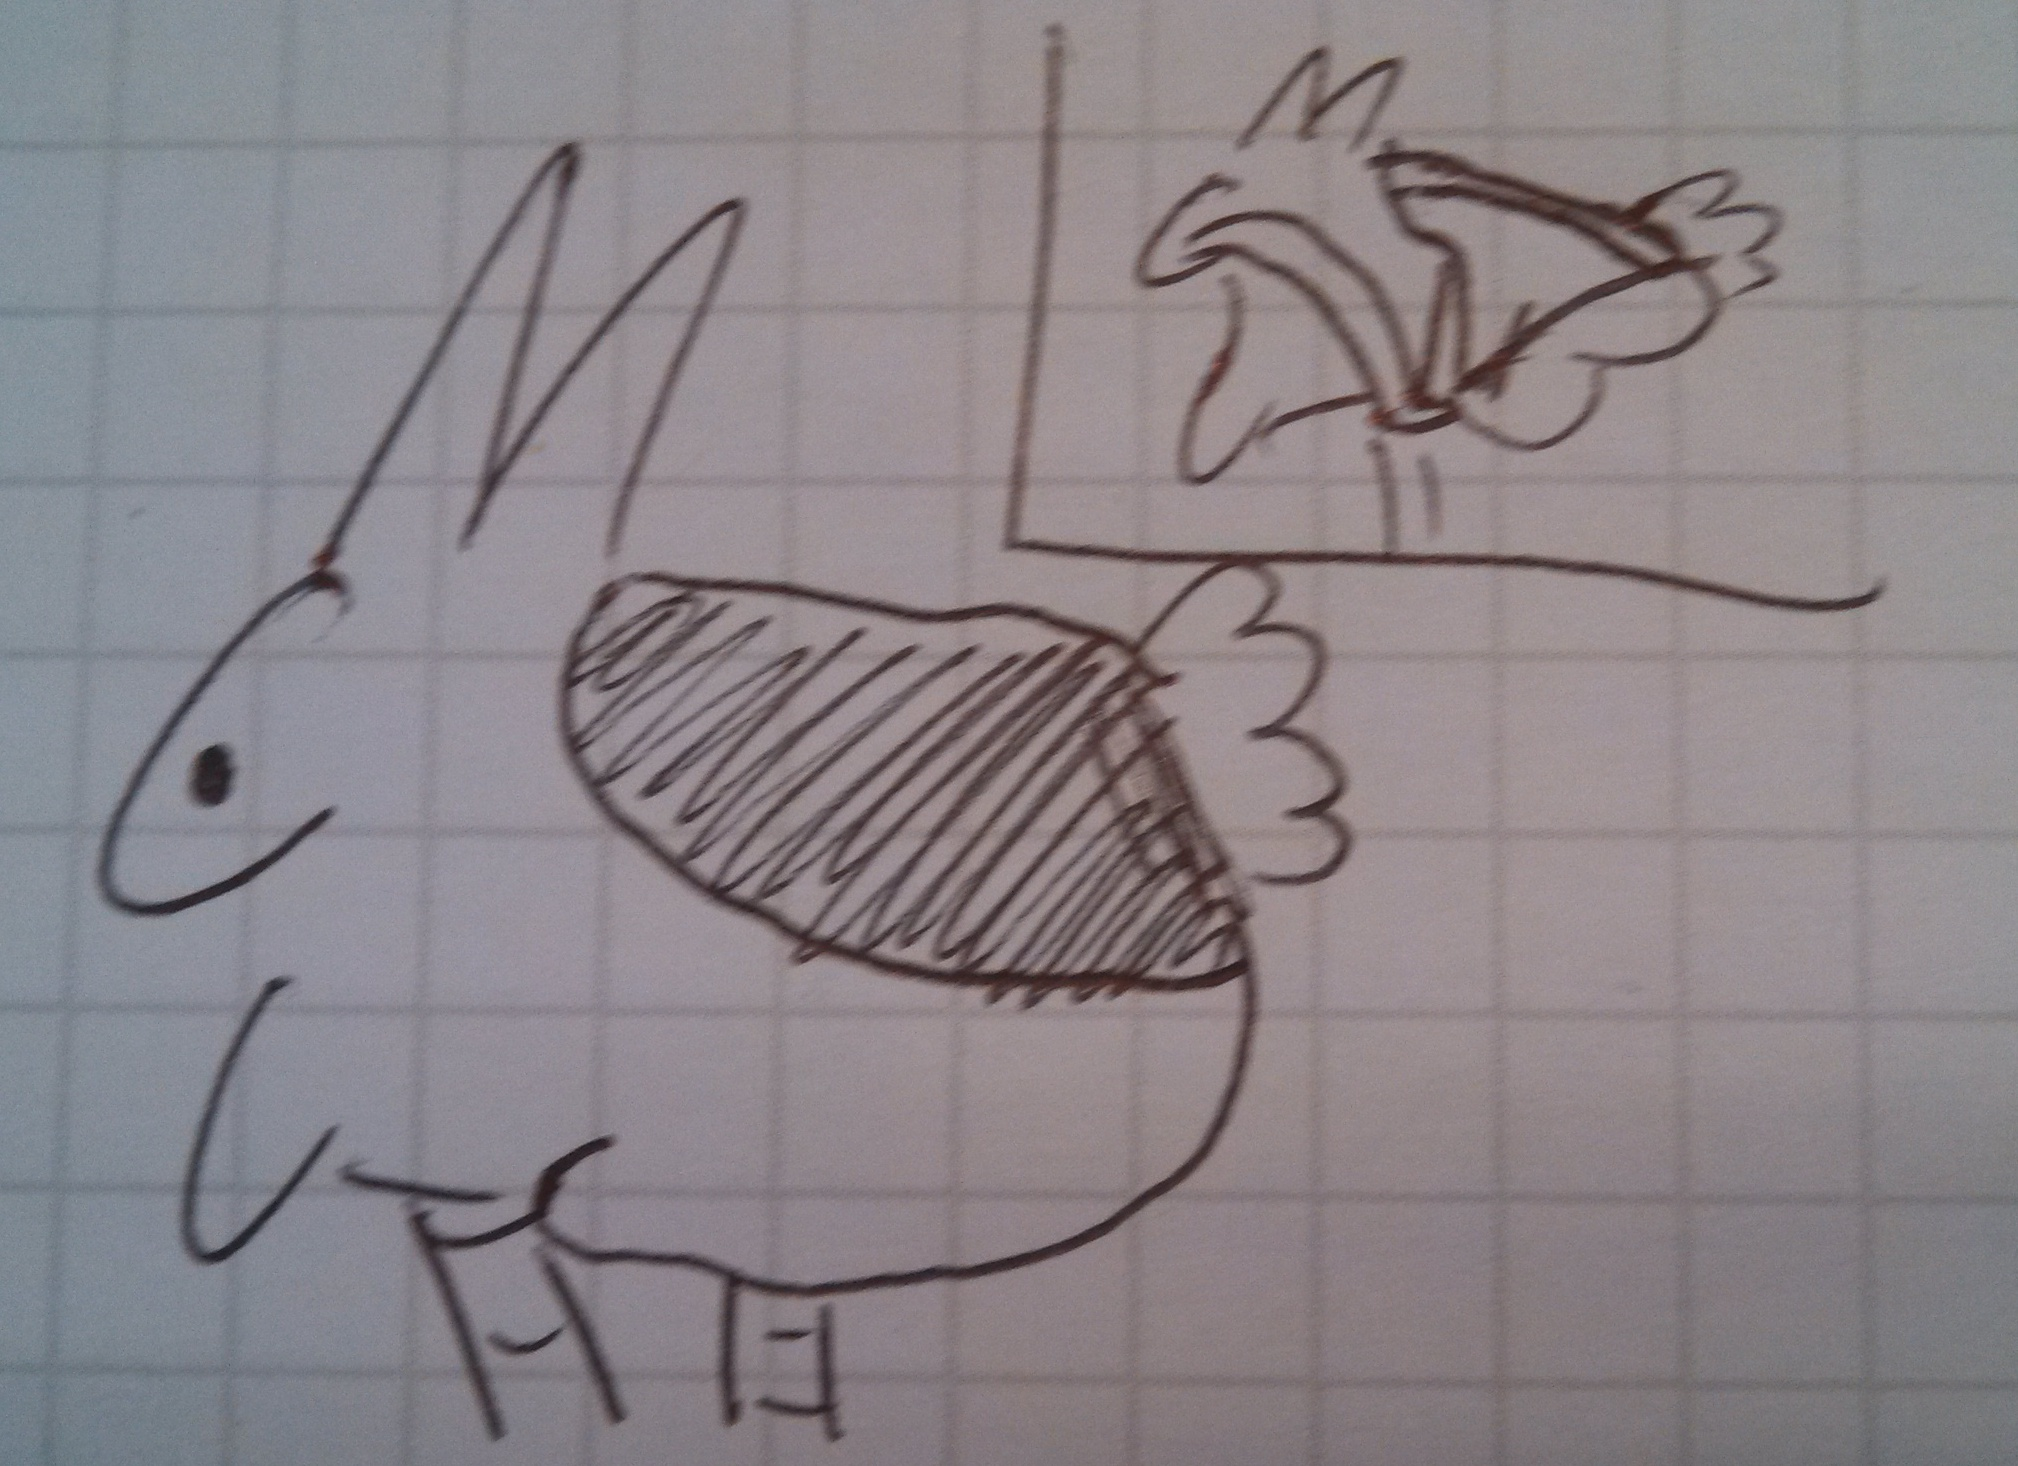
\includegraphics[width=3.4in]{figures/placeholder/bunny.jpg}
\caption{This rabbit has an open tube leading to its mouth and a semi-closed tube capped with flexible material in its back.  When air is sucked in through the open tube, the back becomes stiff as though the rabbit has breathed in.  Inset shows the interior structure.}
\label{fig:breathe}
\end{figure}

We created a rabbit with a pair of tubes that can simulate breathing (see Figure \ref{fig:breathe}).  For this, we used a combination air/vacuum pump: one terminal creates a vacuum while the other creates positive pressure.  Our rabbit has two tubes, one open tube exiting at its mouth and one semi-closed tube capped with rubberlike material in its abdomen.  We connected one tube to each of our pump's terminals, and using a programmable power supply we can mimic a rabbit's breathing pattern.  This example was printed on our Objet Connex 260. \valkyrie{this paragraph is really unclear}

\subsection{Custom Radio}

\begin{figure}[h]
\centering
    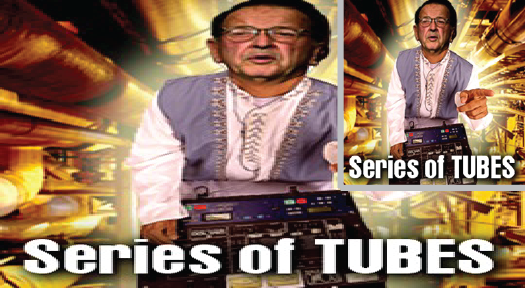
\includegraphics[width=3.4in]{figures/radio.png}
\caption{This radio is assembled from traditional electronic components connected by copper-filled tubes.  The case was designed to allow the components to recess into it slightly.  Inset shows the internal structure of the tubes generated by our design tool.}
\label{fig:radio}
\end{figure}

A custom radio built using tubes allows users to tune to different stations and listen in.  This device uses a network of disconnected open tubes filled with conductive paint to connect traditional electronic components (two potentiometers and a speaker) to a microcontroller (in our case, an Arduino).  We hid the microcontroller and a battery-driven power supply in the base of the radio to make it portable.  For the radio functionality, we attached an Si4703 to the Arduino.  We fabricated this device on our Makerbot Replicator 2.

\subsection{Presence-aware Pen Holder}

\begin{figure}[h]
\centering
    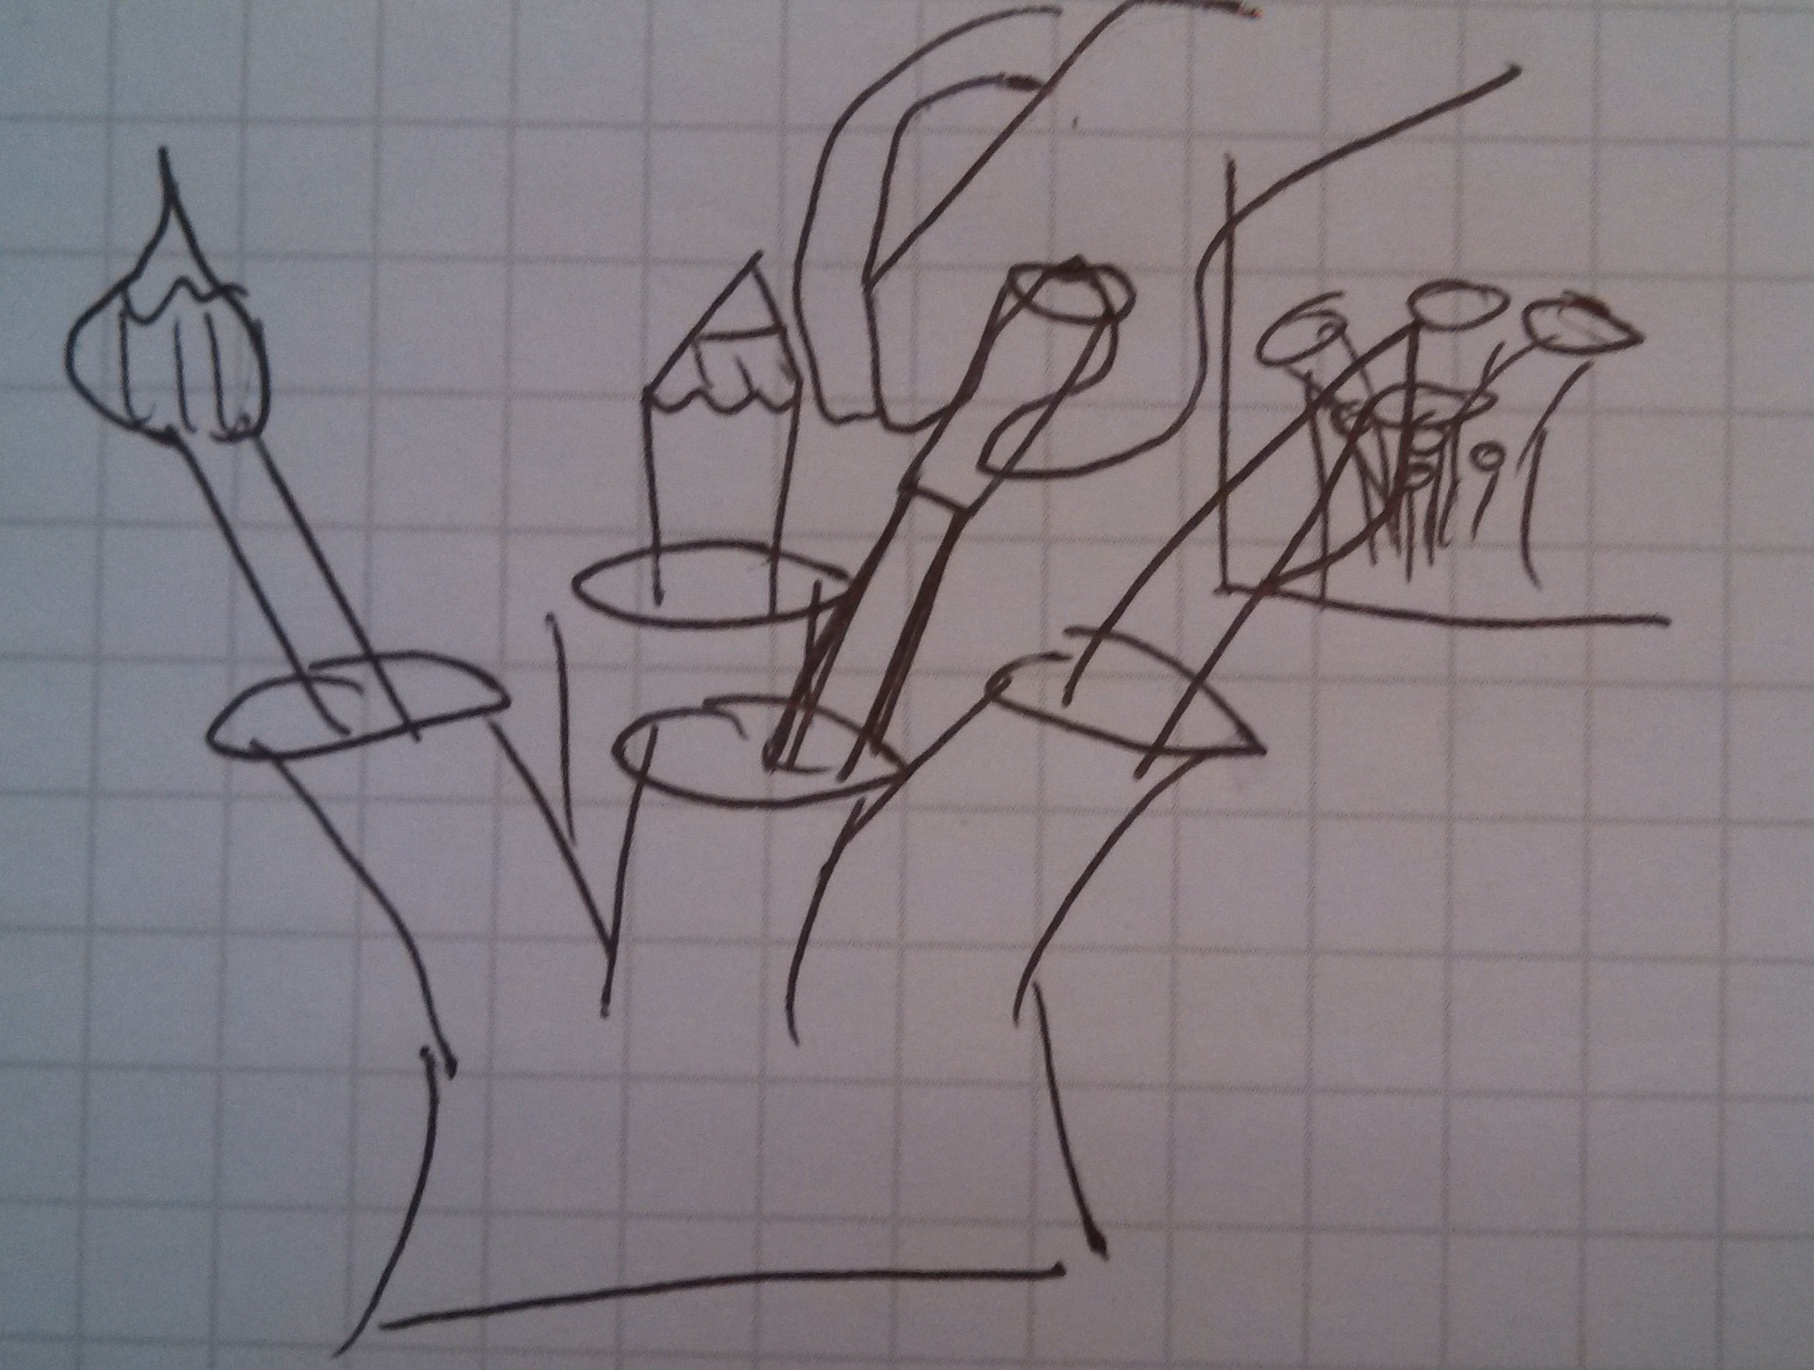
\includegraphics[width=3.4in]{figures/placeholder/pens.jpg}
\caption{This pen holder a modified FlyEye technique to sense the presence or absence of an object in each of its tubes.  Inset shows the internal structure of the tubes generated by our design tool.}
\label{fig:pens}
\end{figure}

Our presence-aware pen holder can distinguish which tool or tools a user has picked up (see Figure \ref{fig:pens}).  Such information was used by \cite{Mueller-constructable} to determine which physical laser pointer a designer was using to interact with their interface.  Our pen holder uses a modification of the FlyEye technique described by Wimmer in \cite{Wimmer-flyeye} and contains open tubes filled with fiber optic cables, one per pen chamber.  Our modification of using a single cable per chamber is possible because we use 6mm diameter fiber optic cables, in comparison to the angel hair tubes used in the original work, and can thus send and receive through the same cable.  At the base of each tube is a QRE1113 line sensor digital breakout board, which has an integrated IR emitter and receiver.   When a pen is in its appointed place, the emitted infrared light is reflected off its bottom and travels back to the receiver, where it registers as bright.  This prototype was built by our Objet Connex 260. \valkyrie{this whole paragraph is unclear}

\subsection{Maze}

\begin{figure}[h]
\centering
    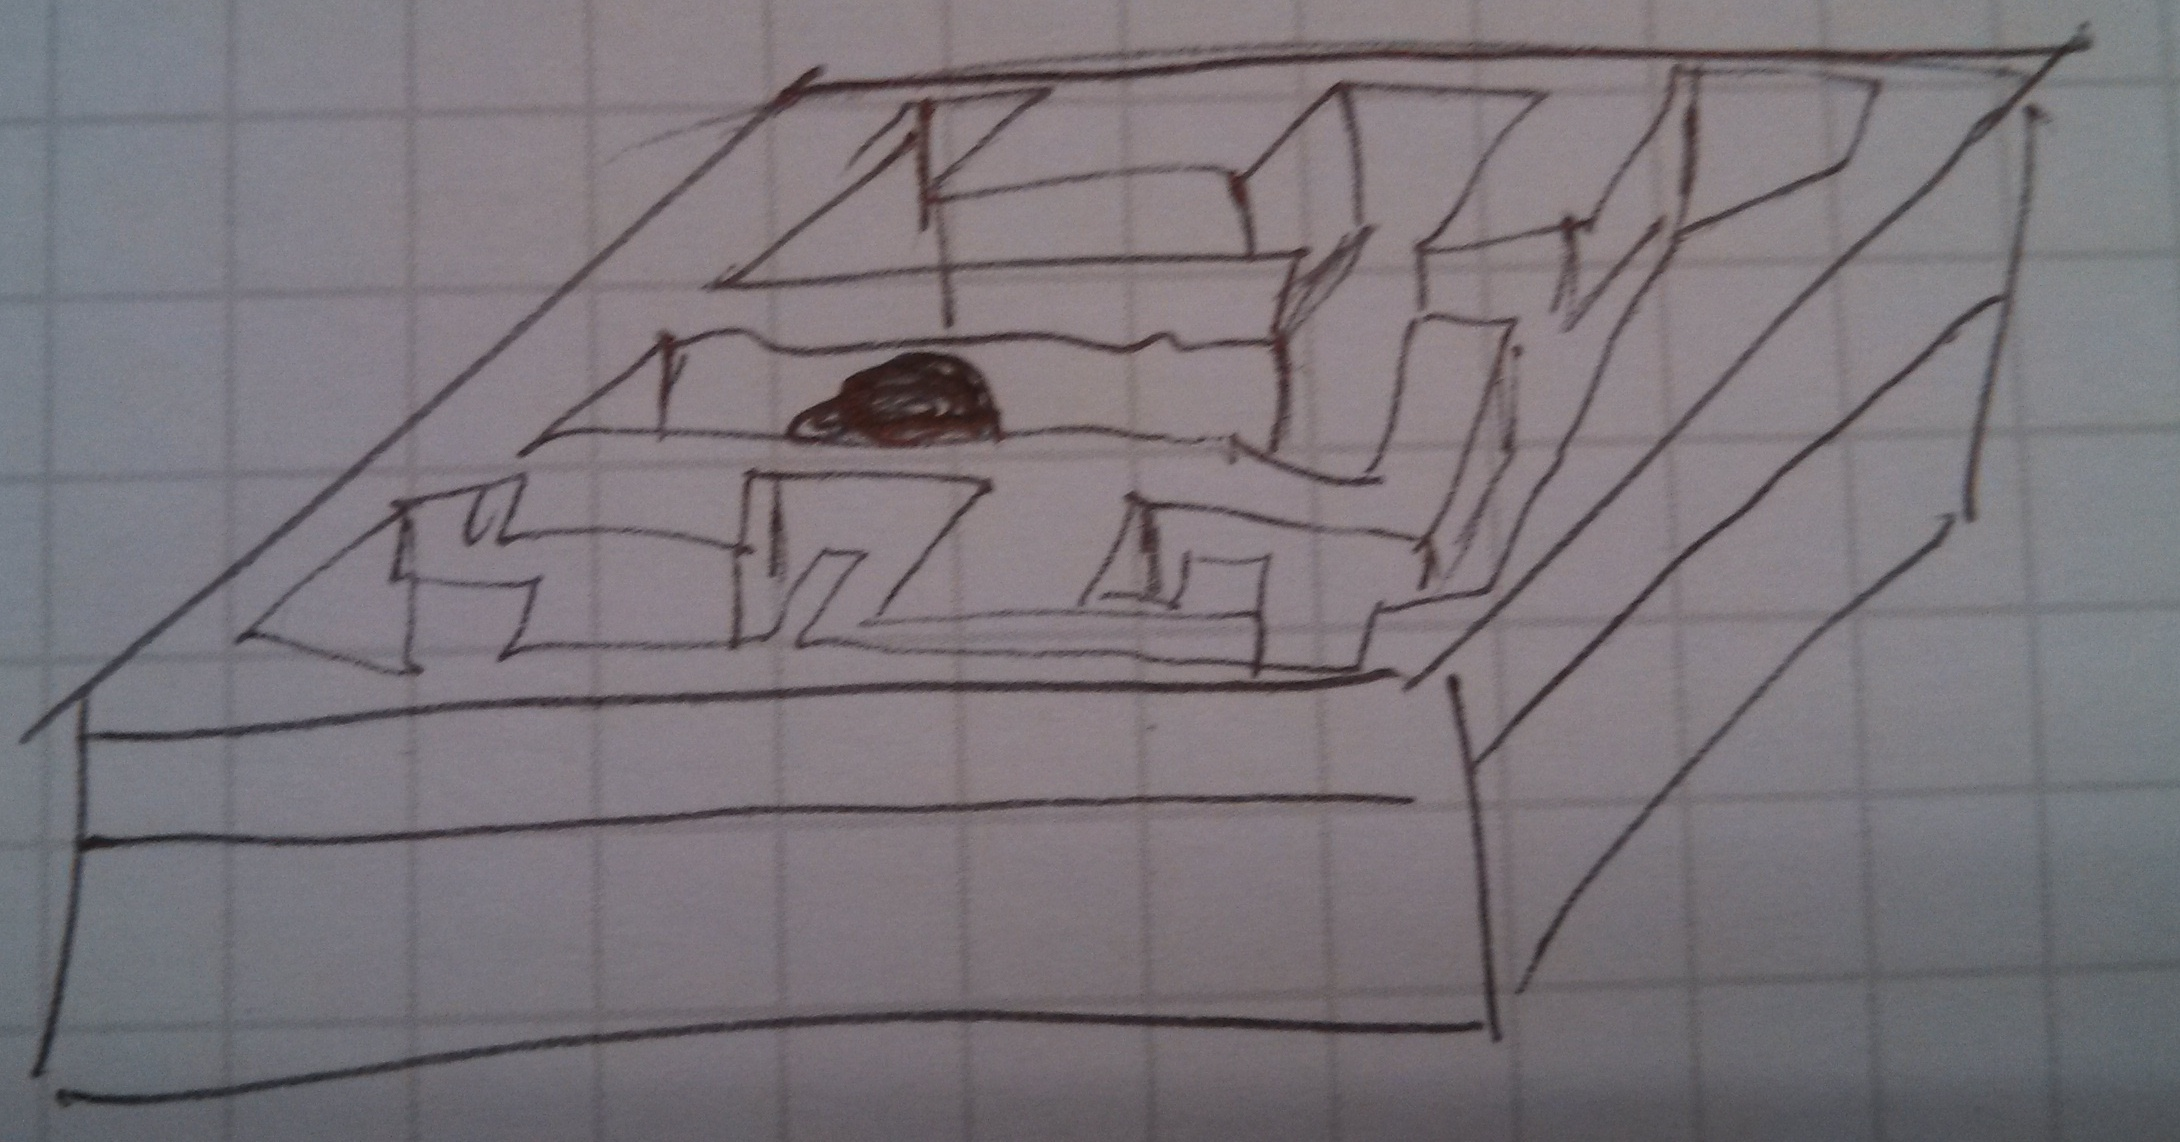
\includegraphics[width=3.4in]{figures/placeholder/maze.jpg}
\caption{Our maze game has a large single particle trapped inside a fully enclosed tube.  It offers hours of fun!}
\label{fig:maze}
\end{figure}

We created a maze game with a single particle trapped in a fully enclosed tube.  To fabricate the tube, we created it in two halves that were fastened together via glue, due to limitations in our ability to remove support material otherwise.  We created this prototype on our Makerbot Replicator 2.

\subsection{Animated Neon Sign}

\begin{figure}[h]
\centering
    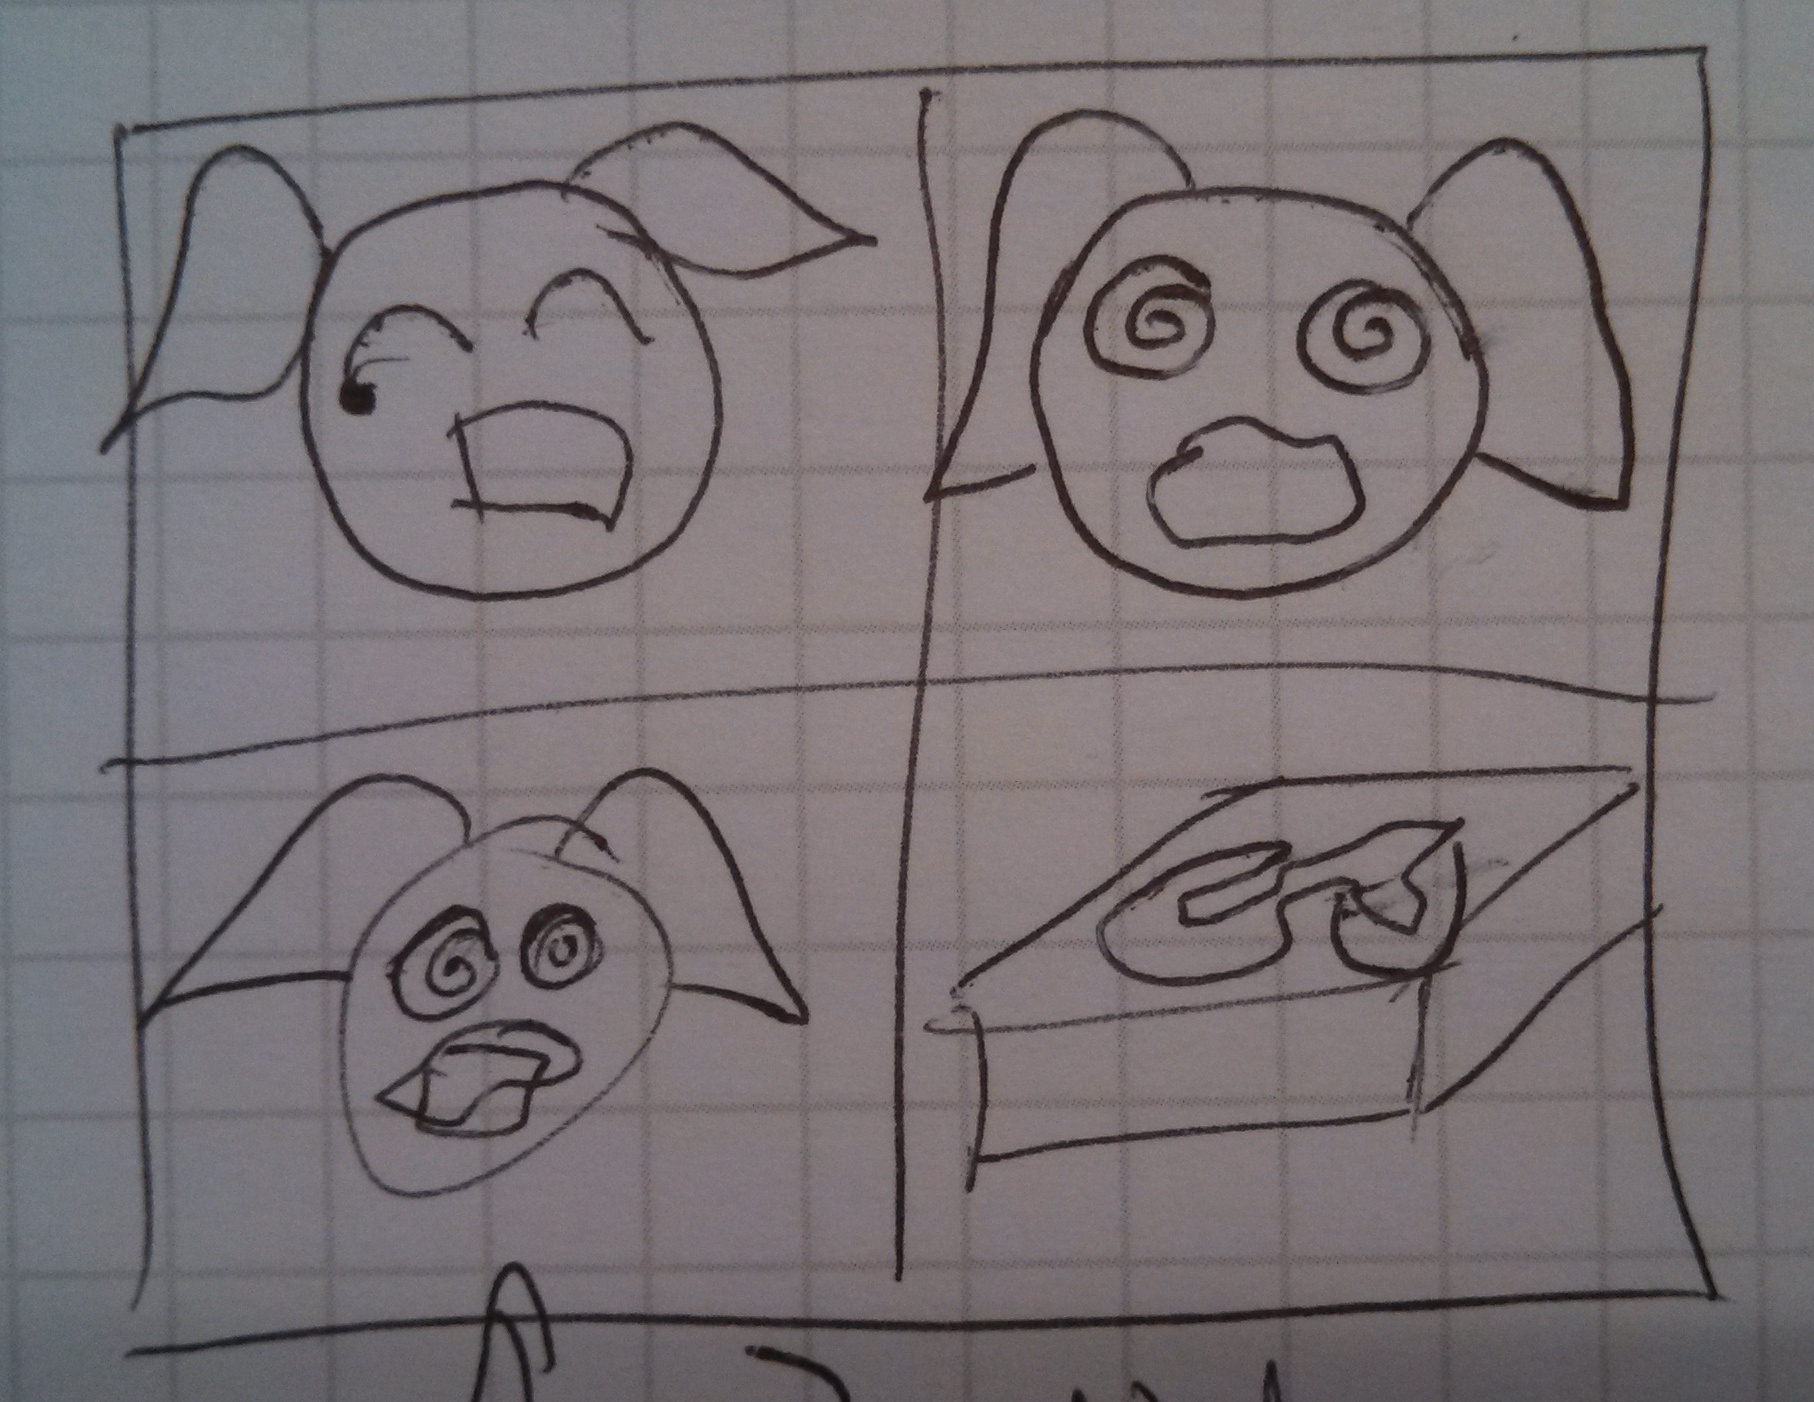
\includegraphics[width=3.4in]{figures/placeholder/sign.jpg}
\caption{A two-state animated neon sign designed using our tool (a)(b) \valkyrie{Tovi: we could use your PDF hax to make this animate in place :)}.  (c) shows the SVG input files to create this sign, and (d) shows an isometric view of the tubes created by our tool. \valkyrie{d) is a lot less interesting if we are making planar tubes.  also, for c, should we show an overlay of the two states?  maybe in different colors?}}
\label{fig:neon}
\end{figure}

Neon art, perhaps best known for its association with Las Vegas, is traditionally made from hand-formed glass tubes containing neon gas.  The tubes light up when a current is passed through them.  For this type of art, the path of the tubes is of crucial importance, as it determines how the sign will look.  We designed a custom neon sign bearing the UIST logo and the waves of Hawaii.  The piece features open tubes due to support-flushing constraints, however the tubes could also be semi-closed (one end must remain open to connect the EL wire to its power source).  They have been threaded with EL wire which is lit in sequence to create an animation.  Our sign was fabricated on the Objet Connex 260.